\documentclass[]{report}
\usepackage{algorithm}
\usepackage[noend]{algpseudocode}
\usepackage{amsmath,amssymb,amsthm,amsfonts}
\usepackage{caption}
\usepackage{comment}
\usepackage{graphicx,verbatim}
\usepackage{listings}
\usepackage{subcaption}

\usepackage[backend=bibtex,style=ieee]{biblatex}
\addbibresource{refs.bib}

\theoremstyle{definition}
\newtheorem{definition}{Definition}[section]

\newcommand{\x}{\mathbf{x}}
\def\bif{\bf if~}
\def\belif{{\bf else if~}}
\def\bthen{{\bf then predict~}}
\def\belse{{\bf else predict~}}

\begin{document}

\title{Accelerating the Search for Certifiably Optimal Rule Lists}
\author{Nicholas Larus-Stone}
\date{3/31/17}
\maketitle

\begin{center}
Abstract
\end{center}

We demonstrate a new algorithm that finds an optimal rule list as well as providing proof of that optimality. Rule lists, which are lists composed of If-Then statements, are similar to decision tree classifiers and are useful because each step in the model's decision making process is understandable by humans. Our algorithm, called CORELS, finds the optimal rule list through the use of three types of bounds: bounds inherent to the rules themselves, bounds based on the current best solution, and bounds based on symmetry between rule lists. We propose novel data structures to minimize the memory usage and runtime of our algorithm on this exponentially difficult problem. One advantage of our algorithm is that it generates not only the optimal rule list and a certificate of optimality, but also the entire solution space of nearly optimal solutions. Our algorithm therefore allows for the analysis and discovery of all optimal and near-optimal solutions on problems requiring human-interpretable algorithms.

\chapter{Introduction}
\label{introduction}

As computing power continues to grow, combinatorial optimization problems that may have been out of the reach of earlier computational power can now be feasibly executed.
The goal of this thesis is to discuss a number of data structure optimizations that allow for the completion of medium to large scale combinatorial optimization problems.
This work builds off of the theoretical bounds and implementation found in Angelino et. al \cite{AngelinoLaAlSeRu17}.
While the techniques found in this thesis are specific to a given machine learning technique, it is our hope that they can be generalized to other combinatorial optimization problems.

We work in the realm of machine learning, specifically focusing on the interpretability of predictive models.
Our algorithm produces models that are highly predictive but in which each step of the model's decision making process can also be understood by humans.
Machine learning models such as neural nets or support vector machines are able to achieve stunning predictive accuracy, but the reasons for these predictions remain unintelligible to a human user.
This lack of interpretability is important because models that are not understood by humans may have hidden bias in their predictive decision making.
A recent ProPublica article found racial bias in the use of a black box machine learning model used for advising criminal sentencing \cite{LarsonMaKiAn16}.
Northepointe, the company which provides COMPAS (the black box model), argues that their use of a black box model is necessitated by the fact that they can achieve better accuracy through the use of that model.
This thesis is part of a body of work that hopes to disprove that statement by showing that it is possible to build interpretable machine learning models without sacrificing accuracy.

To achieve interpretability, we use \emph{rule lists}, also known as decision lists, which are lists comprised of \emph{if-then} statements \cite{Rivest87}. 
This structure allows for predictive models that can be easily interpreted because each prediction is explained by the rule that is satisfied. 
Given a set of rules associated with a dataset, different rule lists can be constructed by placing the rules in different orders.
Since most data points are captured by multiple rules, changing the order of rules leads to different predictions and therefore different accuracies. 
Rule list generation algorithms attempt to maximize predictive accuracy through the discovery of different rule lists.

Generally, interpretable models are viewed as less accurate than black box models.
Thus, proving the optimality of an interpretable model provides an important upper bound on the accuracy of that model.
This helps decision makers decide whether or not to use interpretable models.
In our case, we are searching for the rule list with the highest accuracy----the optimal rule list. 
A brute force solution to find the the optimal rule list would be computationally prohibitive due to the combinatorially number of rule lists.
Our algorithm uses combinatorial optimization to find the optimal rule list in a reasonable amount of time.

Recent work on generating rule lists \cite{LethamRuMcMa15,YangRuSe16} uses probabilistic approaches to generating rule lists.
These approaches achieve high accuracy while also managing to run quickly.
However, despite the apparent accuracy of the rule lists generated by these algorithms, there is no way to determine if the generated rule list is optimal or how close to optimal the rule lists is. 
Our model, called Certifiably Optimal RulE ListS (CORELS), finds the optimal rule list and allows us to also investigate the accuracy of near optimal solutions. 
The benefits of this model are two-fold: firstly, we are able to generate the best rule list on a given data set and therefore will have the most accurate predictions that a rule list can give.
Secondly, since CORELS generates the entire space of potential solutions, we can judge how good rule lists generated by other algorithms are. 
In particular, we can investigate if the rule lists from probabilistic approaches are nearly optimal or whether those approaches sacrifice too much accuracy for speed.
This will allows us to bound the accuracy on important problems and determine if interpretable methods should be used.

CORELS achieves these results by placing a bound on the best performance that a rule list can achieve in the future. 
This allows us to prune that rule list if that bound is worse than the objective value of the best rule list that we have already examined.
We continue to look at rule lists until we have either examined every rule list or eliminated all but one from consideration. 
Thus, when the algorithm terminates, we have found the rule list with the best possible accuracy. 
Our use of this branch and bound technique leads to massive pruning of the search space of potential rule lists and means our algorithm can find the optimal rule list on real data sets.

Due to our interest in interpretability, the amount of data each rule captures informs the value of that rule. 
We want our rule lists to be understandable by humans, so shorter rule lists are more optimal. 
Therefore, we use an objective function that takes into account both accuracy and the length of the rule list to prevent overfitting. 
This means we may not always find the highest accuracy rule list---our optimality is over both accuracy and length of rule lists.
This requires each rule to capture a certain amount of data correctly to make it worth the penalty of making our rule list longer. 
This limits the overall length of our rule lists and prevents us from investigating rule lists containing useless rules.

The exponential nature of the problem means that the efficacy of CORELS is partially dependent on how much our bounds allow us to prune. 
We list a few types of bounds that allow us to drastically prune our search space. 
The first type of bound is intrinsic to the rules themselves.
This category includes bounds such the bound described above that ensures rules capture enough data correctly to overcome a regularization parameter. 
Our second type of bound compares the best future performance of a given rule list to the best solution encountered so far. 
We can avoid examining parts of the search space whose maximum possible accuracy is less than the accuracy of our current best solution. 
Finally, our last class of bounds uses a symmetry-aware map to prune all but the best permutation of any given set of rules.

To keep track of all of these bounds for each rule list, we implemented a modified trie that we call a prefix tree. 
Each node in the prefix tree represents an individual rule; thus, each path in the tree represents a rule list where the final node in the path contains the metrics about that rule list.
This tree structure facilities the use of multiple different selection algorithms including breadth-first search, a priority queue based on a custom function that trades off exploration and exploitation, and a stochastic selection process. 
In addition, we are able to limit the number of nodes in the tree and thereby achieve a way of tuning space-time tradeoffs in a robust manner. 
We propose that this tree structure is a useful way of organizing the generation of rule lists and allows the implementation of CORELS to be easily parallelized.

We applied CORELS to the problem of predicting criminal recidivism on the COMPAS dataset.
Larson et al examines the problem of predicting recidivism and shows that a black box model, specifically the COMPAS score from the company Northpointe, leads to racially biased predictions \cite{LarsonMaKiAn16}.
Black defendants are misclassified at a higher risk for recidivism than occurs in practice, while white defendants are misclassified at a lower risk. 
The model which produces the COMPAS scores is a black box algorithm which is not interpretable, and therefore the model does not provide a way for human input to correct for these racial biases. 
Our model produces accuracies that are similar to standard predictive models and the black-box COMPAS scores while maintaining its interpretability.

CORELS demonstrates a novel approach towards generating interpretable models by identifying and certifying the optimal rule list. 
While searching for that optimal list, we are able to discover near-optimal solutions that provide insight into how effective other interpretable methods might be. 
Rule lists have been around for 30 years \cite{Rivest87}, but computational power has been too limited to attack problems of reasonable scale.
IT is our hope that our tree structure and symmetry-aware map, as well as their associated optimizations, can be applied more broadly to other discrete optimization problems.

Chapter 1 provides an overview of related work in the fields of discrete optimization, interpretable models, and rule lists. 
Chapter 2 proves definitions and explanations of the terminology used in the rest of this thesis.
Chapter 3 describes the implementation and architecture of CORELS, paying special attention to the data structures used to make this problem tractable.
Chapter 4 explains the data structure optimizations performed and the experiments used to validate these optimizations.

\chapter{Related Work}

The use of classification models is popular in a number of different fields from image recognition to churn prediction.
Oftentimes, however, simply receiving a prediction from software is not enough--it is important to have a predictive model that humans can investigate and understand \cite{Ruping06, Bratko97, Quinlan99, Martens11, Freitas14}.
For example, in fields such as medical diagnoses \cite{BellazziZu08} and criminal sentencing \cite{LarsonMaKiAn16}, it is important to be able to investigate the reasons behind a model's predictions.
One reason is that medical experts are unlikely to trust the predictions of these models if they are unable to understand why the model is making certain predictions \cite{Lavrač99}.
Interpretable models also allow users to examine predictions to detect systemic biases in the model.
This is especially important in classification problems such as criminal recidivism prediction where there are often race-related biases\cite{LarsonMaKiAn16} or credit scoring where a justification is necessary for the denial of credit\cite{BaesensMuDeVaSe05}.

Tree structured classifiers are a popular technique that combines interpretability with a high predictive accuracy.
Also called decision trees, these trees are often used as either classification or regression tools.
Every node in the tree classifier splits the data into two subsets; these subsets are then recursively split by nodes lower in the tree.
Nodes are constructed by choosing an attribute that splits the data in such a way that it that minimizes the impurity of each subset.
Trees are constructed by recursively performing splits on the child subsets until the resulting subset is entirely homogenous or small enough.
Methods for constructing decision trees differ primarily based on how they define impurity and therefore what attributes they choose for each node.
In Classification and Regression Trees (CART), Breiman et al lay out an algorithm to create these trees \cite{BreimanFrOlSt84}.
CART tries to minimize Gini impurity which is a measure of the probability that any random element taken from a node is mislabeled.
Another popular algorithm, C4.5, uses the idea of information gain to make its splits instead \cite{Quinlan93}.
In C4.5, nodes are chosen in such a way that each split minimizes the amount of information necessary to reconstruct the original data.
Both algorithms grow the initial tree greedily and then prune later to avoid overfitting.

While most decision trees are constructed greedily, and thus sub-optimally, there has been some work on constructing optimal decision trees \cite{Moret82}.
There has even been the use of a branch and bound technique in an attempt to construct more optimal decision trees.
Garofalakis et al introduce an algorithm to generate more interpretable decision trees by allowing constraints to be placed on the size of the decision tree \cite{GarofalakisHyRaSh00}.
They use the branch-and-bound technique to constrain the size of the search space and limit the eventual size of the decision tree.
During tree construction, they bound the possible Minimum Description Length (MDL) cost of every different split at a given node.
If every split at that node is more expensive than the actual cost of the current subtree, then that node can be pruned.
In this way, they were able to prune the tree while constructing it instead of just constructing the tree and then pruning at the end.
However, even with the added bounds, this approach did not yield globally optimal decision trees because they constrained the number of nodes in the tree.

Whereas decision trees are always grown from the top downwards, decision lists are built while looking at the entire pool of rules.
Thus, while decision trees are often unable to achieve optimal performance even on simple tasks such as determining the winner of a tic-tac-toe game, decision lists can achieve globally optimal performance.
Decision lists are a generalization of decision trees since any decision tree can be converted to a decision list through the creation of rules to represent the leaves of the decision tree \cite{Rivest87}.
Thus, decision list algorithms are a direct competitor to the popular interpretable methods detailed above: CART and C4.5.
Indeed, decision list algorithms are being used for a number of real world applications including stroke prediction \cite{LethamRuMcMa15}, suggesting medical treatments \cite{ZhangLaTsDa2015}, and text classification \cite{LiYa02}.

Work in the field of decision lists focuses both on the generation of new theoretical bounds and the improvement of predictive accuracy of models.
Recent work on improving accuracy has led to the creation of probabilistic decision lists that generate a posterior distribution over the space of potential decision lists\cite{LethamRuMcMa15,YangRuSe16}.
These methods achieve good accuracy while maintaining a small execution time.
In addition, these methods improve on existing methods such as CART or C4.5 by optimizing over the global space of decision lists as opposed to searching for rules greedily and getting stuck at local optima.
Letham et al are able to do this by pre-mining rules, which reduces the search space from every possible split of the data to a discrete number of rules.
We take the same approach towards optimizing over the global search space, though we don’t use probabilistic techniques.
We also want to work in a regime with a discrete number of rules, thus we use the same rule mining framework from Letham et al to generate the rules for our data sets.
This framework creates features from the raw binary data and then builds rules out of those features.
Yang et al builds on this earlier work by placing additional bounds on the search space and creating a fast low-level framework for computation, specifically a high performance bit vector manipulation library.
We use that bit vector manipulation library to help perform computations involving calculating accuracy of rules.

Our use of a branch and bound technique is inspired by the fact that it is often applied to problems that have a large number of potential solutions without a polynomial time algorithm.
The branch and bound algorithm recursively splits the data into subgroups, yielding a tree-like structure.
Then, by calculating a value corresponding to the end goal of the algorithm (e.g. accuracy), some branches of the tree can be proved to be worse in every case than another branch and therefore can be pruned, reducing the search space.
This technique has been used to solve NP-hard problems such as the Traveling Salesman Problem \cite{LittleMuSwKa63}, the Knapsack Problem \cite{Kolesar67}, or the Mixed Integer Programming problems \cite{Clausen99}.
Branch and Bound is also used as an optimization technique for some machine learning algorithms, though it has not been applied to decision lists before now \cite{ChapelleSiKe06}.

\chapter{Definitions}\label{ch:definitions}
\newthought{We present definitions and explanations} of concepts and terms that are used throughout this work.

\section{Rules}
A \textit{rule} is an IF-THEN statement consisting of a boolean antecedent and a classification label.
We are working in the realm of binary classification, so the label is either a 0 or a 1.
The boolean antecedents are generated from the rule mining mechanism and are a conjunction of boolean features.
These antecedents are satisfied by some data points (also called \textit{samples}) and not for others.
We say a rule \textit{classifies} a given data point when the antecedent is satisfied for that data point.
As we combine these rules into rule lists, only the first rule that classifies any given data point can make a prediction for that data point.
Thus, we say a rule \textit{captures} a given data point if it is the first rule in a rule list to classify that data point.

\section{Rule Lists}
%Let us define a training dataset of size N as $\{x_n, y_n\}_{n=1}^N$ where each $x_n \in \{0, 1\}^J$ are binary features and each $y_n \in \{0, 1\}$ are binary labels.
%Each rule $x_n$ therefore classifies some of the data points (those indices where $x_{n, j} = 1$).
%Define a rulelist $\mathbf{r} = (r_1, r_2, ... , r_k, r_0)$ where each $r_i \in \{x_n\}_{n=1}^N, \forall i > 0$.
%$r_0$ is defined as the default rule, which makes a prediction on all data points that are not captured in rules $1 ... k$. 
A \textit{rule list} is an ordered collection of rules.
As defined above, rules have an inherent accuracy based on what data they classify and how they predict the label.
When they are placed into a rule list, however, their accuracy is based on what data they capture---which is usually not the same as what data they classify.
They can perform better or worse than their inherent accuracy depending on what rules come before them in a given rule list.
Thus, our algorithm is focused on finding the list composed of the best rules and the order that maximizes predictive accuracy.
A rule list also has a \textit{default rule}, placed at the end of all of these rules, that classifies all data points and predicts the majority label.
This allows a rule list to make predictions for all points because any point not captured by the pre-mined rules is therefore captured by the default rule.
We refer to the set of rules that compose a rule list, not including the default rule, as a \textit{prefix}.

\begin{figure}[t!]
%\vspace{-3mm}
\begin{algorithmic}
\normalsize
\State \bif $(age=23-25) \wedge (priors=2-3)$ \bthen $yes$
\State \belif $(age=18-20)$ \bthen $yes$
\State \belif $(sex=male) \wedge (age=21-22)$ \bthen $yes$
\State \belif $(priors>3)$ \bthen $yes$
\State \belse $no$
\end{algorithmic}
%\vspace{-3mm}
\caption{An example rule list that predicts two-year recidivism for the COMPAS dataset, found by CORELS.}
\label{fig:rule-list}
\end{figure}

\section{Objective Function}
Rule lists have a loss function based on the number of points that are misclassified by the rules in the rule list.
We define our \textit{objective} function to be the sum of that loss and a regularization term.
We use a \textit{regularization} term, which is a constant times the length of the rule list.
This has the effect of preventing overfitting on training data sets as well as preventing extremely long, and therefore uninterpretable, rule lists.
While the objective is related to accuracy (a higher accuracy means a lower objective), we will be optimizing over the objective function instead of just the accuracy in order to get the benefits of the regularization term.

\begin{math}
objective(RL) = loss(RL) + c * len(RL)
\end{math}

\section{Bounds}\label{sec:bounds}
For a set of $n$ rules, there are $n!$ possible rule lists.
Finding the optimal rule list using a brutal force is infeasible for any problem of reasonable size.
Our algorithm uses the discrete optimization technique of branch-and-bound to solve the combinatorially difficult problem of finding an optimal rule list.
This requires tight bounds that allow us to prune as much of the search space as possible.
These bounds are formalized and proved in Angelino et al. \cite{AngelinoLaAlSeRu17} and are reproduced in Appendix A.
For clarity we present informal summaries of the important bounds here.

\subsection{Lower Bound}
We use the term \textit{lower bound} to mean the best possible outcome for the objective function for a given prefix.
We do this by calculating the error of the prefix and assuming that any points uncaptured by the prefix will be predicted correctly.
This is equivalent to assuming that the default rule captures all points perfectly.
Because any future extensions of the prefix can only ever make mistakes, we will be able to use it to prune our exploration.
An important property of the lower bound is that it increases monotonically.

\subsection{Hierarchical Objective Bound}
The main bound for our algorithm is the \textit{hierarchical objective bound}. 
It says that we do not need to purse a rule list if it has a lower bound that is worse than the best objective we have already seen.
This follows from the fact that lower bounds increase monotonically, so if the lower bound of rule list A is worse than the objective of rule list B, any extensions of rule list A can never be better than rule list B.
This allows us to prune large parts of the search space by not pursuing rule lists that could never be better than something we've already seen.

\begin{figure}
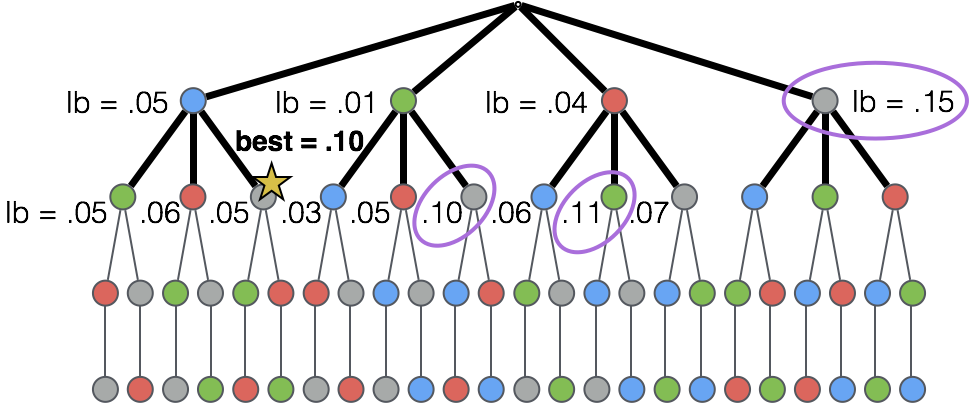
\includegraphics[width=0.5\textwidth]{figs/ela_branch-and-bound-tree.png}
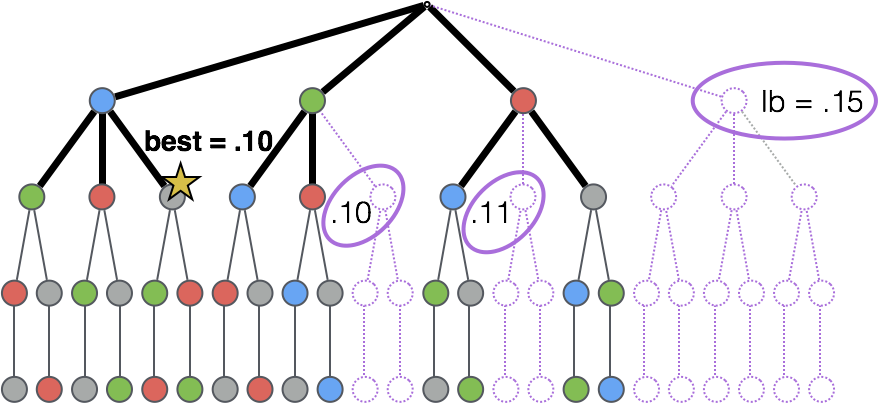
\includegraphics[width=0.5\textwidth]{figs/ela_branch-and-bound-tree-pruned.png}
\caption[Objective bound]{This tree shows the hierarchical objective bound in action. Our best objective seen is the prefix (blue, gray) with an objective of $0.10$. Any prefixes with lower bound greater than this objective--(gray), (red, green), (green, gray) can be pruned and not ever looked at.
\label{fig:objective-bound}}
\end{figure}

\subsection{Permutation Bound}

As defined above, every sample is captured by precisely one rule--any sample that is caught by rule A in the rule list AB cannot be caught by rule B. 
Now consider a \textit{permutation} of the rule list AB: the rule list BA.
Any samples that are captured by either rule A or B but not both will be captured identically in both rule lists.
Samples that are captured by both rules will again be captured the same in both rule lists, though they may be predicted differently in the two rule lists.
Thus, regardless of the order in which the rules appear, rule lists AB and BA will capture exactly the same set of data.
They will differ only in which rules capture which samples, so their accuracy may differ. 
We can use this knowledge to create a bound as follows.
If we know that the lower bound of AB is better than the lower bound of BA, we can eliminate from consideration all rule lists beginning with BA.
This is due to the fact that any corresponding rule list beginning with AB will capture exactly the same samples as the equivalent rule list beginning with BA but will have a better objective score.
We can eliminate all but one permutation of a given set of rules using this principle.

\begin{figure}
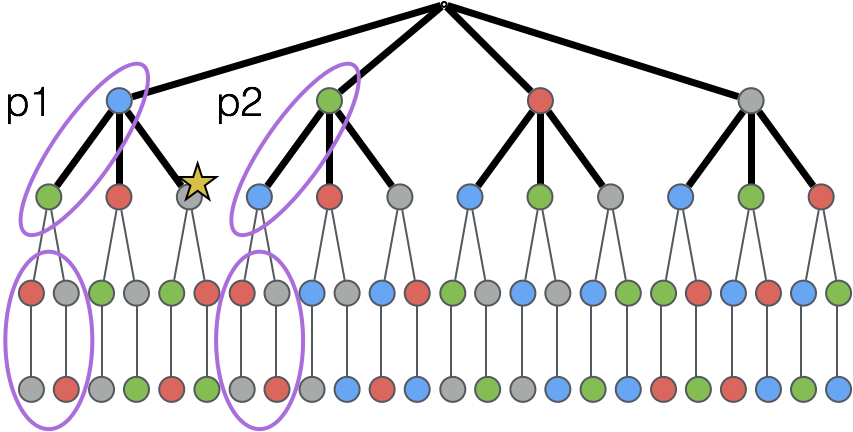
\includegraphics[width=0.5\textwidth]{figs/ela_branch-and-bound-permutations.png}
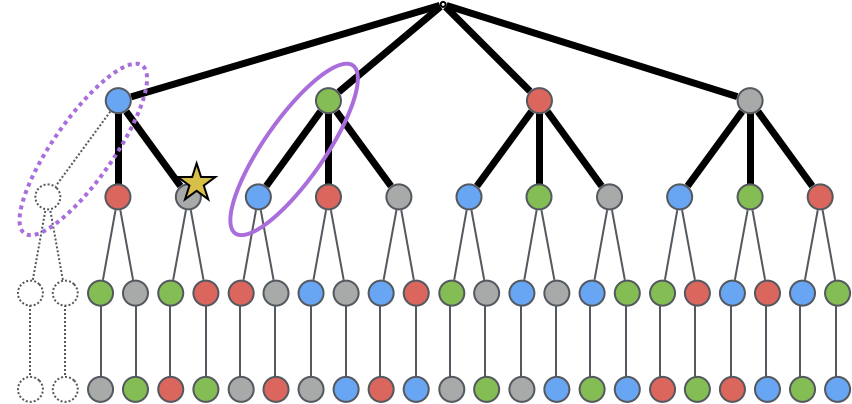
\includegraphics[width=0.5\textwidth]{figs/ela_branch-and-bound-permutations-pruned.png}
\caption[Permutation bound]{This tree shows the use of the permutation bound. Prefixes (blue, green) and (green, blue) are permutations of each other, so their lower bounds can be compared. The prefix (green, blue) has a better lower bound, so (blue, green) can be pruned and none of its children have to be examined.
\label{fig:permutation-bound}}
\end{figure}

\subsection{Support Bounds}
Due to our regularization term in calculating our objective function, adding a rule that does little to help our accuracy will actually be harmful to the overall objective score.
This allows us to place bounds that rely on the \textit{support} of the rules we add.
It never makes sense to add a rule that increases the objective function, so we only consider adding rules that capture enough points correctly to overcome the regularization penalty.
By definition, rules that don't capture enough of the remaining points cannot capture them correctly, so this provides us with two closely related bounds.
As our rule lists get longer many rules do not capture enough points that haven't already been captured and this bound begins to play an even larger role.

\subsection{Equivalent Points Bound}
This bound relies on the structure of our dataset.
In our dataset, we may encounter two data points that have the same features but different labels.
We call the set of these data points \textit{equivalence points}, and describe the label that occurs less often as the \textit{minority} label.
Any rule that classifies one point in an equivalence class will also classify all other points in that class.
However, it is impossible to correctly predict equivalence points with different labels using a single rule.
So, for a given class of equivalence points, we know that we will mispredict all of the points with a minority label.
We can thus update our lower bound to be tighter than just assuming that the default rule will capture all remaining points correctly.
Now, we assume all remaining points will be captured incorrectly if it is an equivalent point with a minority label.
This gives us much tighter lower bounds and in practice allows us to prune much more efficiently.

\section{Curiosity}
There are a number of different ways to explore the search space (see \ref{sec:queue}).
Some methods, such as BFS, prioritize exploration---looking at all rule lists of a given length before proceeding to the next length.
Others, such as a priority queue ordered by lower bound, focus on purely exploiting the best prefixes that we've seen.
We define a new metric, \textit{curiosity}, that blends together both exploration and exploitation.
Curiosity is a function of both the lower bound and the number of samples captured.
This prioritizes rule lists that still have many samples left to capture (exploration) while also pursuing rule lists with promising lower bounds (exploitation).

\begin{math}
curiosity(RL) = lowerBound(RL) - c * (len(RL) - 1)  * (nsamples / |captured(RL)|)
\end{math}

\section{Remaining Search Space}
One metric for tracking the efficacy of our optimizations will be seeing how quickly we reduce the remaining search space.
We start with a combinatorially large search space, but quickly prune it down using our bounds.
We calculate the remaining search space is by looking at all of the potential prefixes in our  queue and seeing how much each prefix could potentially be expanded.
Due to our regularization term, we are able to bound the maximum length of a prefix as our best objective gets updated.
This upper bound on the maximum length of a viable prefix allows us to place an upper bound on the search space as well.
We find that the remaining search space decreases rapidly at the beginning of execution, then slowly decreases until the very end of execution when it again rapidly decreases.

This chapter lays out the design and implementation of the system used to generate optimal rule lists. 
We begin by describing each of the three main data structures used to run our algorithm--a prefix trie, a symmetry-aware map, and a queue. 
Then, we 

\section{Prefix Trie}
The prefix trie is a custom C++ class and is used as a cache to keep track of rule lists we have already evaluated. 
Each node in the trie contains the metadata associated with that corresponding rule list. 
This metadata includes bookkeeping information such as what child rule lists are feasible as well as information such as the lower bound and prediction for that rule list.
In addition to our base trie class, we implemented two different node types that we use in our algorithm.
First, we implemented a class that has an additional field that tracks the curiosity of a given prefix as defined in \ref{ch:definitions}.
Curiosity is used by our queue to determine the order that prefixes are explored.
Since the curiosity field is just a double, the memory overhead is minimal and the speed-up of using curiosity as opposed to BFS is sizable (see \ref{exp:priority}).
We also implemented a class that has an additional field keeping track of the captured vector for that prefix.
This captured vector has length $nsamples$, which means it is memory expensive.
However, using the captured vector allows us to speed up our incremental computations because we would otherwise have to recompute this vector every time we used that prefix.

\section{Queue}\label{sec:queue}
Our queue support many different types of search policies that we can use to explore the search space.
We implement a number of different scheduling schemes including BFS, DFS, various priority metrics, and a stochastic exploration process.
Due to our use of incremental computation, our queue contains pointers to leaves in the trie.
The search process involves selecting which leaf node to explore.
The stochastic exploration process bypasses the use of a queue by performing random walks on the trie until a leaf is reached.
Our other scheduling schemes use a STL C++ priority queue to hold and order all of the leaves of the trie that still need to be explored.
Our priority metrics can be ordered by curiosity, the objective of a prefix, or the lower bound of a prefix.
We find that using an exploitation strategy such as ordering by curiosity or lower bound will usually lead to a faster runtime than using BFS.

In C++ the priority queue is a wrapper container that prevents access to the container underlying the queue.
Therefore we cannot access elements in the middle of the queue, even if we have know the value that we're trying to access..
Thus, we run into a problem where we may delete something in the prefix trie that is currently in the queue but have no way to update the queue.
We deal with this by lazily marking nodes as deleted in the prefix trie without deleting the physical node until it has been popped off of the queue.
As Fig \ref{fig:queue_gc} shows, this leads to a situation where our logical queue is actually smaller than the physical queue.

\begin{figure}[t!]
\begin{center}
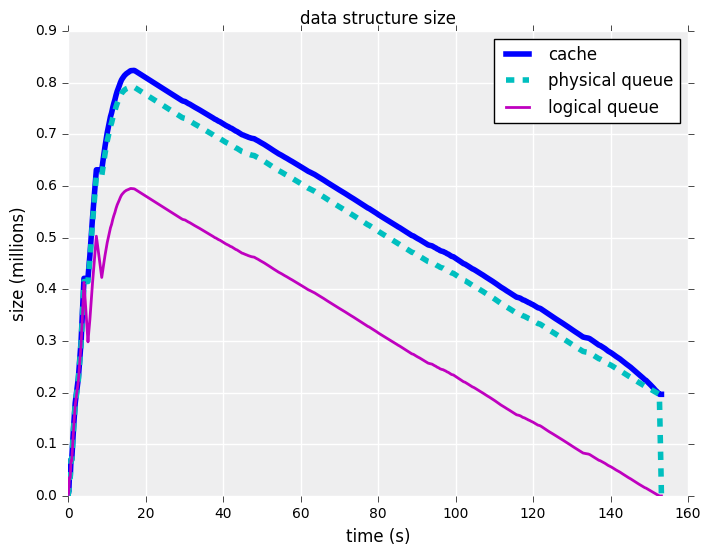
\includegraphics[width=0.65\textwidth]{figs/compas-queue-cache-size-insertions.png}
\end{center}
\caption{Size of prefix trie, logical queue, and physical queue over the execution of our algorithm. Note that the gap between the logical queue and the physical queue is due to our lazy garbage collection}
\label{fig:queue_gc}
\end{figure}

\section{Symmetry-aware map}
We implement our symmetry-aware map as an STL unordered\_map.
We use this data structure to implement the permutation bound described in \ref{def:perm-bound}.
We have two different versions of the map with different key types that allow permutations to be compared and pruned.
In both cases, the values consist of the best lower bound and the actual ordering of the rules that is best for that permutation.
In the first version, keys to the map are represented as the canonical order of the rules: i.e. the lists 3-2-1 and 2-3-1 both map to 1-2-3.
The second version has keys that represent the captured vector.
Our earlier permutation bound was based off of the fact that different permutations capture the same data, so this type of key will again be equivalent for the rule lists 3-2-1 and 2-3-1.
Representing keys with captured vectors could potentially match more permutations since two prefixes may not be permutations of each other but might capture the same data points and therefore fall under the permutation bound.
In fact, we find that this occurs only rarely, as the number of rule lists examined is only slightly less in the captured vector case.
Despite only supporting one bound, the permutation map plays a significant role in our memory usage.

\begin{figure}[t!]
\begin{center}
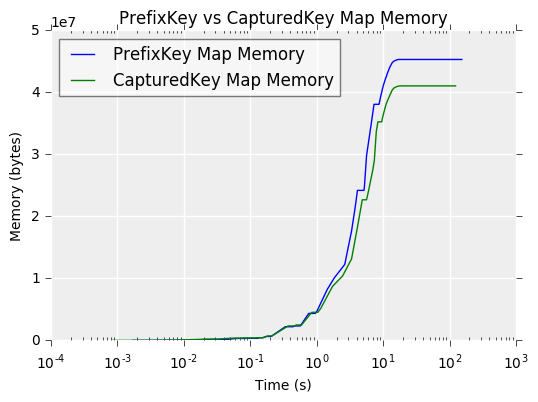
\includegraphics[width=0.4\textwidth]{figs/prefix-captured_pmap_mem.png}
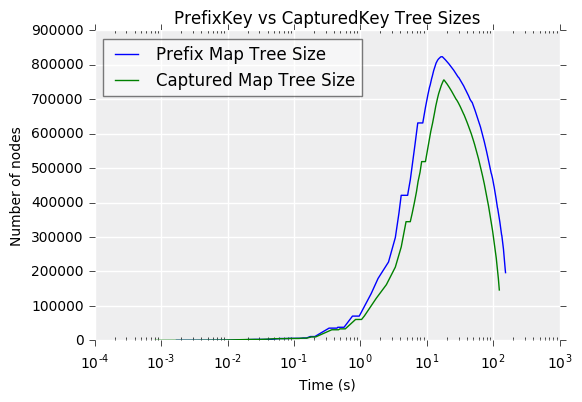
\includegraphics[width=0.4\textwidth]{figs/prefix-captured_tree_size.png}
\end{center}
\caption{This graph shows the memory usage of the map when using CapturedKeys and PrefixKeys. We see that CapturedKeys provide minimal space savings over PrefixKeys due to the slight decrease in nodes inserted into the trie.}
\label{fig:prefix-captured}
\end{figure}


\section{Incremental execution}
We detail the execution of our program below.
Our program ends when all leaves of the trie have been explored and there is nothing else in our queue.
We can also choose to not receive the full certificate of optimality by exiting execution when a certain number of rule lists are in the trie.
While there are still leaves of the trie to be explored, we use our scheduling policy to select the next rule list to evaluate.
Then, for every rule that is not already in this parent rule list, we calculate the lower bound, objective, and other metrics for the potential child rule list consisting of the new rule appended to the parent rule list.
We check the support bounds, the hierarchal objective bound, the permutation bound, and the lookahead bound.
If the child rule list has a lower bound that is better than all of these bounds, then we insert it into the permutation map, the tree, and the queue and update the minimum objective if necessary.
Otherwise, we do not insert it into any of our data structures and we continue to the next potential rule to add, having excluded a rule list from being optimal.
After evaluating all the rules we could add to our parent rule list, we return to the main loop and look at the next leaf of the trie.

\begin{algorithm}[t!]
  \caption{Branch-and-bound for learning rule lists}
\label{alg:branch-and-bound}
\begin{algorithmic}
\normalsize
\State \textbf{Output:} Outputs the best rule list and its objective\\
\State $opt \gets NULL$
\State $T \gets initializeTree()$
\State $Q \gets queue(\,[T.root()\,])$
\State $P \gets map(\{\})$
\While {$Q$ not empty}
	\State $node \gets Q$.pop(\,)
	\State $oldObj \gets T$.minObjective(\,)
	\State incremental($node, T, Q, P$) \Comment{Evaluate all of node's children}
	\If {$T$.minObjective(\,) $< oldOb$j}
		\State $opt \gets T$.bestRuleList(\,)
		\State $T$.garbageCollect(\,)
	\EndIf
\EndWhile
\State \Return $opt, T$.minObjective(\,)
\end{algorithmic}
\end{algorithm}

\begin{algorithm}[t!]
  \caption{Incremental evaluation of a prefix}
\label{alg:incremental}
\begin{algorithmic}
\normalsize
\State \textbf{Input:} Node to be evaluated~$parent$,
prefix tree~$T$,
queue~$Q$,
symmetry-aware map~$P$
\State \textbf{Output:} None---destructively updates best objective in the tree\\
\State $prefix \gets parent$.prefix(\,)
\State $t \gets c *$ nsamples \Comment{This forms the threshold for our support bounds}
\For {$rule \notin prefix$}
	\State $rlist \gets prefix$.append($rule$)
	\State $cap \gets parent\text{.notCaptured(\,)} \wedge rule$.notCaptured(\,)
	\If {$|cap| < t$} \Comment{Minimum support bound}
		\State continue
	\EndIf
	\State $capZero \gets cap \wedge T$.zeroLabel(\,) \Comment{Record how many zeros the new rule captures}
	\State $corr \gets max\{|capZero|, |cap| - |capZero|\}$
	\If {$corr < threshold$} \Comment{Minimum correct support bound}
		\State continue
	\EndIf
	\State $lb = parent.\text{bound(\,)} - parent.\text{minority(\,)} + \frac{|cap| - corr}{nsamples} + c$ \Comment{Calculate lower bound}
	\If {$lb  >= T.$minObjective(\,)} \Comment{Objective bound}
		\State continue
	\EndIf
	\State $notCap \gets parent\text{.notCaptured(\,)} \wedge \neg cap$
	\State $notCapZero \gets notCap \wedge T$.zeroLabel(\,)
	\State $defaultCorr \gets max\{|notCapZero|, |notCap - notCapZero|\}$
	\State $obj \gets lb + \frac{|notCap| - defaultCorr}{nsamples}$ \Comment{Calculate objective}
	\If {$obj < T$.minObjective(\,)} \Comment{Update minimum objective}
		\State $T.minObjective(obj)$
	\EndIf
	\If{$lb + c >= T.$minObjective(\,)} \Comment{Lookahead bound---don't add to queue if its children will all be worse than the minimum objective}
		\State continue
	\EndIf
	\State $n \gets P.insert(rlist)$ \Comment{Symmetry-aware map handles permutation bound for us}
	\If {$n$} \Comment{$n$ will be NULL if it failed the permutation bound check}
		\State $T.$insert($n$)
		\State $Q.$push($n$)
	\EndIf
\EndFor
\end{algorithmic}
\end{algorithm}

\section{Garbage Collection}
Every time we update the minimum objective, we garbage collect on the trie.
We do this by traversing from the root to all of the leaves.
Any time we encounter a node with a lower bound larger than the minimum objective, we delete its entire subtree.
In addition, if we encounter a node with no children, we prune upwards---deleting that node and recursively traversing the tree towards the root, deleting any childless nodes.
This garbage collection allows us to limit the memory usage of the trie.
In practice, though, the minimum objective is not update that often, so garbage collection is triggered only rarely.

\section{Templates vs Inheritance}
Our system has a lot of different modular parts--various priority metrics, symmetry-aware map types, and different types of information stored in trie nodes.
Since we were using C++, we took advantage of its templating system to achieve this modularity.
We believed that it would be the easiest way to switch out different components of the system, but did not think about the ramifications of this choice.
Due to code duplication, large amount of templates can lead to a much larger execution.
Indeed, with a pure templating system, our executable was 253732 bytes.

Our other alternative way to maintain modularity was to take advantage of C++'s class system and use inheritance and polymorphism.
Now, instead of having a template argument for each data structure, we can have a base data structure type and then implement each of our extensions as subclasses.
Therefore, we can write all of our functions to take the base class as arguments and then pass in the specialized subclasses based on command line arguments.
This requires the use of virtual functions, which are potentially a bit slower than regular functions because they require a vtable lookup.
With a pure inheritance framework, our executable was 171288 bytes.
However, even with the inheritance framework, the runtime of our algorithm was not significantly different from the template runtime.
Thus, since inheritance provided a much cleaner code base to work with, we decided to switch to an inheritance based framework.

\section{Memory tracking}
We track memory through the use of C++11 custom allocators.
Our allocators are simple malloc wrappers that also log which data structure the allocation is coming from--the trie, the map, or the queue.
We validated the accuracy of this memory tracking by running the program under Valgrind's massif heap profiler tool and comparing the outputs.
Our outputs matched Valgrind's to within a few hundred bytes, so we concluded that our memory tracking was successful.
The heap profiling of Valgrind has a large overhead, while our memory logging is more limited and therefore overhead is very minimal.
This allows us to write out our memory usage per data structure on a regular basis without incurring the large overhead of Valgrind.

\chapter{Experiments}

\section{Symmetry-aware Map Optimization}
As one of our two main data structures, the memory usage of our symmetry-aware map is something that was very important to us.
We found that we often had trouble running large data sets because we would run out of memory before certifying the optimal rule list.
In these long runs, our permutation map would grow to be hundreds of thousands or millions of entries large.
Thus, carrying a lot of memory overhead with each node led to serious memory bloat and ran us out of memory.
This section explores some of the techniques we used to handle this memory bloat.

Our symmetry-aware map was originally an STL map with keys as STL sets of size\_t and values as pairs of STL vectors of size\_t and a double.
The first problem is that the STL map is implemented as a red-black tree, meaning every node had the overhead of multiple pointers pointing to its children.
This can be solved using a STL unordered map, which is implemented as a hashtable.
That has some overhead, since it will allocate more buckets than are filled, but nowhere near to the two pointers per node of overhead of the STL map.

Next, the representation of the rule ids no longer had to be size\_t.
We made an assumption that we'll never have more than 65000 rules, so we used unsigned shorts for our rule ids.
This means that our final data structure was able to use only 2 bytes per rule id instead of 8 bytes for a size\_t.
Since we're keeping two different representations of the prefix--the canonical order and the actual order of the prefix, and these prefixes can be of length on the order of 5 rules, saving 6 bytes per rule translates to a lot of 

Our initial implementation used an STL set as the key, which carries a lot of overhead because of all the operations that a set needs to support.
For a prefix of length 6, the corresponding key therefore takes up 
After starting with the STL set, we transition to a sorted STL vector.
This reduced overhead because a vector is essentially just an array with a little bit of overhead.
However, all of these STL containers support a broader range of operations than we needed.
All we needed was some way to compare the canonical orders and determine if they were the same.
We eventually achieved this simply by allocating a chunk of memory that held the length of the prefix and the sorted order of the ids.
This means that, for a prefix of length 6, we use 14 bytes for the key.

We had a similar set of issues with our values for the permutation map.
Beginning with a STL vector to keep track of the actual order of the rules in the prefix, we again wanted to remove the overhead incurred by the fact that STL containers need to support a wider array of operations than we needed.
Thus, we could use a similar technique to what we did with the keys to keep track of the prefix order.
However, in fact, we can do even better because we already have a canonical representation of the rules--all we need in the value was the ordering of those rules.
Thus, we can use unsigned chars instead of unsigned shorts to record the index of where the rules in the canonical order are in the prefix.

However, these optimizations all pertained to the symmetry-aware map with prefix keys.
Dealing with the captured vector keys required a different approach.
Our captured vectors were of type mpz, and since unordered\_map requires a custom hash for unsupported types, we had to find a way around that.
STL has some hash functions for built in types, so we initially wrote a function to convert between our VECTOR type and a $std::vector<bool>$.
This conversion turned out to be very slow, especially as we were running on data sets with many samples, meaning these mpz types were fairly memory intensive.
Once we wrote our own hash function and were able to use our mpz type again, it became much faster.

\section{Ablation--how much does each bound/optimization help?}

We ran a number of experiments where we only took out one component and measured the effects on the time and memory of our algorithm.
We find that each optimization and bound is extremely important to concluding the algorithm quickly and in a reasonable amount of memory.
These were all executed on a MacBook Air with 8GB of RAM.

\subsection{Full CORELS system}

Running the full CORELS system on the COMPAS dataset yields the optimal solution and its certificate within 121s.

\begin{figure}[t!]
\begin{center}
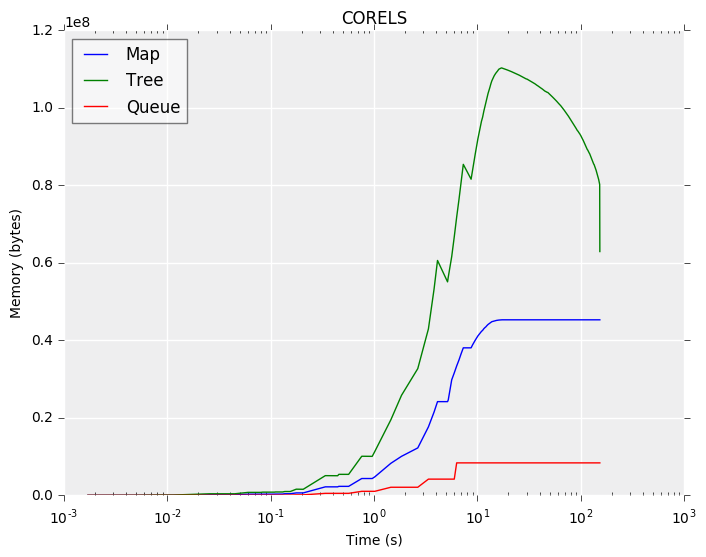
\includegraphics[width=0.4\textwidth]{figs/corels_mem.png}
\end{center}
\caption{}
\label{fig:prefix-captured}
\end{figure}

\subsection{Priority Queue} \label{exp:priority}
142.s

\subsecton{Support Bounds}
261s

\subsection{Symmetry-aware map}

\subsection{Lookahead Bound}

\subsection{Equivalent points bound}

\subsection{Objective Bound}

\section{Parallelization}
The tree structure of our trie lends itself nicely to parallelization.

We began by trying to parallelize the inner loop of our incremental evaluation.
This 
This had too much contention.

Instead, we can parallelize the search over the tree itself.

\begin{comment}
\section{Methodology}

\subsection{Improving Memory Usage of Symmetry-aware Map and Trie (Finding memory bottlenecks)}

Fixing the memory bloat of the symmetry aware map

$tt = ./bbcache -c 1 -n 100000 -p 1 -r 0.001 ../data/tdata\_R.out ../data/tdata\_R.label$
$tt_{reg} = ./bbcache -c 1 -n 100000 -p 1 -r 0.01 ../data/tdata\_R.out ../data/tdata\_R.label$

$bc = ./bbcache -c 1 -n 100000 -p 1 -r 0.001 ../data/bcancer.out ../data/bcancer.label$
$bc_{reg} = ./bbcache -c 1 -n 100000 -p 1 -r 0.01 ../data/bcancer.out ../data/bcancer.label$
$bc_{nodes} = ./bbcache -c 1 -n 1000000 -p 1 -r 0.001 ../data/bcancer.out ../data/bcancer.label$

$ad = ./bbcache -c 1 -n 100000 -p 1 -r 0.001 ../data/adult\_R.out ../data/adult\_R.label$
$ad_{reg} = ./bbcache -c 1 -n 100000 -p 1 -r 0.001 ../data/adult\_R.out ../data/adult\_R.label$
$ad_{nodes} = ./bbcache -c 1 -n 100000 -p 1 -r 0.001 ../data/adult\_R.out ../data/adult\_R.label$

\subsubsection{Keys as $std::set<size\_t>$, vals as $std::pair<std::vector<size\_t>, double>$}

\begin{center}
\begin{tabular} { |c|c|c|c|c|c|c| }
\hline
Name & \multicolumn{2}{c|}{Perm Map} & \multicolumn{2}{c|}{Tree} & time & accuracy \\
\hline
tt & 24928104 & 79.8\%  & 6317856 & 20.2\% & 17.601315 & 1.00000 \\

$tt_{reg}$ & 105849872 & 79.6\% & 27170304 & 20.4\% & 47.910126 & 1.00000 \\

bc &109281024 & 91.9\% & 9622752 & 8.1\% & 4.901384 & 0.98682 \\

$bc_{reg}$ & 197476840 & 74.9\% & 66004224 & 25.1\% & 438.309378 & 0.95168 \\

$bc_{nodes}$ & 1173870840 & 92.4\% & 96021408 & 7.6\% & 54.334499 & 0.98682 \\

ad & 36083664 & 79.0\% & 9614400 & 21.0\% & 4.485328 & 0.81048 \\

$ad_{reg}$ & 42119256 & 81.4\% & 9600768 & 18.6\% & 3.735894 & 0.81081 \\

$ad_{nodes}$ & 443942192 & 82.2\% & 96007296 & 17.8\% & 73.517540 & 0.81078 \\
\hline
\end{tabular}
\end{center}

\subsubsection{Keys as $std::vector<size\_t>$, vals as $std::pair<std::vector<size\_t>, double>$}

REPLACE NUMBERS

\begin{center}
\begin{tabular} { |c|c|c|c|c|c|c| }
\hline
Name & \multicolumn{2}{c|}{Perm Map} & \multicolumn{2}{c|}{Tree} & time & accuracy \\
\hline
tt & 24928104 & 79.8\%  & 6317856 & 20.2\% & 17.601315 & 1.00000 \\

$tt_{reg}$ & 105849872 & 79.6\% & 27170304 & 20.4\% & 47.910126 & 1.00000 \\

bc &109281024 & 91.9\% & 9622752 & 8.1\% & 4.901384 & 0.98682 \\

$bc_{reg}$ & 197476840 & 74.9\% & 66004224 & 25.1\% & 438.309378 & 0.95168 \\

$bc_{nodes}$ & 1173870840 & 92.4\% & 96021408 & 7.6\% & 54.334499 & 0.98682 \\

ad & 36083664 & 79.0\% & 9614400 & 21.0\% & 4.485328 & 0.81048 \\

$ad_{reg}$ & 42119256 & 81.4\% & 9600768 & 18.6\% & 3.735894 & 0.81081 \\

$ad_{nodes}$ & 443942192 & 82.2\% & 96007296 & 17.8\% & 73.517540 & 0.81078 \\
\hline
\end{tabular}
\end{center}

\subsubsection{Keys as $std::vector<unsigned short>$, vals as vals as $std::pair<std::vector<unsigned short>, double>$}

\begin{center}
\begin{tabular} { |c|c|c|c|c|c|c| }
\hline
Name & \multicolumn{2}{c|}{Perm Map} & \multicolumn{2}{c|}{Tree} & time & accuracy \\
\hline

tt & 7701812 & 57.1\%  & 5791368 & 42.9\% & 14.315976 & 1.00000 \\

$tt_{reg}$ & 36875368 & 59.4\% & 25160784 & 40.6\% & 42.896435 & 1.00000 \\

bc & 22464444 & 71.8\% & 8820856 & 28.2\% & 2.526981 & 0.98682 \\

$bc_{reg}$ & 77240290 & 56.1\% & 60503872 & 43.9\% & 404.327822 & 0.95168 \\

$bc_{nodes}$ & 230106908 & 72.3\% & 88019624 & 27.7\% & 27.476015 & 0.98682 \\

ad & 15292352 & 63.4\% & 8819800 & 36.6\% & 4.213340 & 0.81048 \\

$ad_{reg}$ & 16277360 & 64.9\% & 8811968 & 35.1\% & 3.525658 & 0.81081 \\

$ad_{nodes}$ & 160178964 & 64.5\% & 88161568 & 35.5\% & 47.643006 & 0.81078 \\
\hline
\end{tabular}
\end{center}

\subsubsection{Unordered map--Keys as $std::vector<unsigned short>$, vals as vals as $std::pair<std::vector<unsigned short>, double>$}

\begin{center}
\begin{tabular} { |c|c|c|c|c|c|c| }
\hline
Name & \multicolumn{2}{c|}{Perm Map} & \multicolumn{2}{c|}{Tree} & time & accuracy \\
\hline

tt & 7423740 & 56.2\%  & 5791368 & 43.8\% & 13.609930 & 1.00000 \\

$tt_{reg}$ & 35661696 & 58.6\% & 25160784 & 41.4\% & 42.945947 & 1.00000 \\

bc & 21698948 & 71.1\% & 8820856 & 28.9\% & 2.138304 & 0.98682 \\

$bc_{reg}$ & 72839418 & 54.6\% & 60503872 & 45.4\% & 359.959682 & 0.95168 \\

$bc_{nodes}$ & 227288484 & 72.1\% & 88019624 & 27.9\% & 21.061545 & 0.98682 \\

ad & 14746584 & 62.6\% & 8819800 & 37.4\% & 3.402276 & 0.81048 \\

$ad_{reg}$ & 15641304 & 64.0\% & 8811968 & 36.0\% & 3.106825 & 0.81081 \\

$ad_{nodes}$ & 159236876 & 64.4\% & 88161568 & 35.6\% & 43.151872 & 0.81078 \\
\hline
\end{tabular}
\end{center}

\subsubsection{Unordered map--Keys as $unsigned short *$, vals as vals as $std::pair<std::vector<unsigned short>, double>$}

\begin{center}
\begin{tabular} { |c|c|c|c|c|c|c| }
\hline
Name & \multicolumn{2}{c|}{Perm Map} & \multicolumn{2}{c|}{Tree} & time & accuracy \\
\hline

tt & 5539628 & 48.9\%  & 5791368 & 51.1\% & 16.437973 & 1.00000 \\

$tt_{reg}$ & 28019470 & 52.7\% & 25160784 & 47.3\% & 40.594612 & 1.00000 \\

bc & 16164866 & 64.7\% & 8820856 & 35.3\% & 2.175347 & 0.98682 \\

$bc_{reg}$ & 56388394 & 48.2\% & 60503872 & 51.8\% & 371.937364 & 0.95168 \\

$bc_{nodes}$ & 168402474 & 65.7\% & 88019624 & 34.3\% & 19.322026 & 0.98682 \\

ad & 12403876 & 58.4\% & 8819800 & 41.6\% & 3.230369 & 0.81048 \\

$ad_{reg}$ &12987184 & 59.6\% & 8811968 & 40.4\% & 2.809433 & 0.81081 \\

$ad_{nodes}$ & 131981438 & 60.0\% & 88161568 & 40.0\% & 43.882791 & 0.81078 \\
\hline
\end{tabular}
\end{center}

\subsubsection{Above (3.1.5) and reordering tree nodes}

\begin{center}
\begin{tabular} { |c|c|c|c|c|c|c| }
\hline
Name & \multicolumn{2}{c|}{Perm Map} & \multicolumn{2}{c|}{Tree} & time & accuracy \\
\hline

tt & 5539620 & 51.3\%  & 5264880 & 48.7\% & 15.787402 & 1.00000 \\

$tt_{reg}$ & 28019462 & 55.1\% & 22873440 & 44.9\% & 35.468984 & 1.00000 \\

bc & 16164858 & 66.8\% & 8018960 & 33.2\% & 1.933180 & 0.98682 \\

$bc_{reg}$ & 56388386 & 50.6\% & 55003520 & 49.4\% & 345.475240 & 0.95168 \\

$bc_{nodes}$ & 168402466 & 67.8\% & 80017840 & 32.2\% & 19.360888 & 0.98682 \\

ad & 12403868 & 60.7\% & 8018000 & 39.3\% & 3.121322 & 0.81048 \\

$ad_{reg}$ & 12987176 & 61.8\% & 8010880 & 38.2\% & 2.703331 & 0.81081 \\

$ad_{nodes}$ & 131981430 & 62.2\% & 80146880 & 37.8\% & 37.732368 & 0.81078 \\
\hline
\end{tabular}
\end{center}

\subsubsection{Unordered map--Keys as $unsigned short *$, vals as vals as $std::pair<double, unsigned char*>$}

\begin{center}
\begin{tabular} { |c|c|c|c|c|c|c| }
\hline
Name & \multicolumn{2}{c|}{Perm Map} & \multicolumn{2}{c|}{Tree} & time & accuracy \\
\hline

tt & 3655508 & 41.0\%  & 5264880 & 59.0\% & 13.046520 & 1.00000 \\

$tt_{reg}$ & 20377236 & 47.1\% & 22873440 & 52.9\% & 52.318813 & 1.00000 \\

bc & 10630776 & 57.0\% & 8018960 & 43.0\% & 2.184780 & 0.98682 \\

$bc_{reg}$ & 39937362 & 42.1\% & 55003520 & 57.9\% & 399.382231 & 0.95168 \\

$bc_{nodes}$ & 109516456 & 57.8\% & 80017840 & 42.2\% & 21.461987 & 0.98682 \\

ad & 10113288 & 55.8\% & 8019680 & 44.2\% & 3.390032 & 0.81048 \\

$ad_{reg}$ &10333056 & 56.3\% & 8010880 & 43.7\% & 3.096620 & 0.81081 \\

$ad_{nodes}$ & 104855160 & 56.7\% & 80150800 & 43.3\% & 43.222397 & 0.81078 \\
\hline
\end{tabular}
\end{center}

\subsubsection{Ordered map--Keys as $std::vector<bool>$, values as $std::vector<unsigned short>, double$}

\begin{center}
\begin{tabular} { |c|c|c|c|c|c|c| }
\hline
Name & \multicolumn{2}{c|}{Perm Map} & \multicolumn{2}{c|}{Tree} & time & accuracy \\
\hline

tt & 11413638 & 68.4\%  & 5274016 & 31.6\% & 14.426219 & 1.00000 \\

$tt_{reg}$ & 55946962 & 69.3\% & 24777016 & 30.7\% & 42.086578 & 1.00000 \\

bc & 14602388 & 62.3\% & 8822616 & 37.7\% & 266.859001 & 0.98829 \\

$bc_{reg}$ & 125912468 & 68.7\% & 57428448 & 31.3\% & 295.119223 & 0.95168 \\

$bc_{nodes}$ & 126686680 & 58.9\% & 88285032 & 41.1\% & 4430.965258 & 0.98829 \\

ad & 267807290 & 96.8\% & 8804224 & 3.2\% & 71.885551 & 0.81078 \\

$ad_{reg}$ & 356845610 & 97.6\% & 8816632 & 2.4\% & 53.843208 & 0.81081 \\

$ad_{nodes}$ & 1018150922 & 97.4 \% & 88000704 & 2.6 \% & 7005.960590 &  0.81078\\
\hline
\end{tabular}
\end{center}

\subsubsection{Ordered map--Keys as $VECTOR$, values as $std::vector<unsigned short>, double$}

\begin{center}
\begin{tabular} { |c|c|c|c|c|c|c| }
\hline
Name & \multicolumn{2}{c|}{Perm Map} & \multicolumn{2}{c|}{Tree} & time & accuracy \\
\hline

tt & 5791368 & 61.3\%  & 3658580 & 38.7\% & 10.644521 & 1.00000 \\

$tt_{reg}$ & 25160784 & 55.2\% & 20380308 & 44.8\% & 33.295206 & 1.00000 \\

bc & 10641520 & 54.7\% &8820856 & 45.3\% & 0.914455 & 0.98682 \\

$bc_{reg}$ & 60503872 & 60.2\% & 39948106 & 39.8\% & 309.314620 & 0.95168 \\

$bc_{nodes}$ & 109527200 & 55.4\% & 88019624 & 44.6\% & 11.085341 & 0.98682 \\

ad & 10115616 & 53.4\% & 8821648 & 46.6\% & 3.169979 & 0.81048 \\

$ad_{reg}$ & 10335384 & 54.0\% & 8811968 & 46.0\% & 2.126727 & 0.81081 \\

$ad_{nodes}$ & 104857488 & 54.3 \% & 88165880 & 45.7 \% & 38.948489 &  0.81078\\
\hline
\end{tabular}
\end{center}

 ./bbcache -c 1 -n 10000000 -p 1 -r 0.01 ../data/compas.out ../data/compas.label ../data/compas.minor
TREE mem usage: 355815632, max mem usage: 749862630
PMAP mem usage: 161689645, max mem usage: 188028213
QUEUE mem usage: 16384, max mem usage: 32760

\subsection{Parallelizing Execution}

file:///Users/nlarusstone/Downloads/eur-few-cs-95-04.pdf

Begin by trying to run multiple threads on a stochastic selection algorithm.

Initially coarse locking on the entire tree--share both the tree and permutation map in memory
No--actually no permutation map, no locking, no garbage collection
	Threadpool to run the evaluate children (because that's where the majority of work is done)
	Locking is causing a lot of contention and is difficult to get reliable results

Can't parallelize the for loop inside evaluate children
	Without synchronization, turns out that the insertion of a child into its parent's children\_ map can lead to a null access if the underlying tree rebalances
	Synchronization causes too much contention on that lock, so will want our threads to be working on different parts of the tree instead of trying to speed up calculations for a single prefix

Partition tree from top
	Each worker starts with (nrules/num\_threads) rules in its tree and then it can add whatever rules it would like after that.

\subsection{How much does each bound help? (Finding time bottlenecks)}

\subsection{Investigating similarity of prefixes}

\subsection{Cached bit vector node}

\subsection{Exploration of nearly-optimal rule lists and comparisons to other algorithms}

\subsection{Inheritance vs Templating}


With pure templates:
Executable size: 253732
-c 1 -n 100000 -p 1 -r 0.001 ../data/tdata\_R.out ../data/tdata\_R.label: 11.191856
-c 1 -n 100000 -p 1 -r 0.001 ../data/bcancer.out ../data/bcancer.label: 1.188271
-c 1 -n 100000 -p 1 -r 0.001 ../data/adult\_R.out ../data/adult\_R.label: 2.906099
-c 1 -n 100000 -p 1 -r 0.001 ../data/compas.out ../data/compas.label: 4.038996

$10^7$ nodes
9.822864 8.850554 8.943174
77.118279 68.101442 63.307958
416.428278 399.025332 404.614529
427.698726 427.517602 410.294034

$10^7$ (Commented out logger)
8.705810 (8.829541)
58.472542 (53.311810)
372.558429 (249.713447)
398.003311 (103.392936)

Inherited queue:
Executable size: 249484
9.461418
1.324893
3.158447
4.354028

Inherited queue + pmap:
Executable size: 209876
9.192366
1.068136
3.257429
4.484909

$10^7$ nodes
8.968495 9.562288 10.391837
70.315091 66.474482 70.032368
395.544781 388.303023 402.497634
448.220752 508.278413 453.807489

Pure Inheritance:
Executable size: 171288
$10^7$ nodes
13.433584 12.546750
64.704144 60.598935
200.708991 187.573605
127.951469 111.120107

Logger with return statements:
9.263342
60.493697
203.016282
110.914362

With NullLogger (no-op virtual functions):
8.918576
55.236019
185.749401
105.225227

With Logger as an inherited class:
9.039654
56.637848
190.003558
107.623293
\end{comment}

\subsection{Applications: COMPAS, Medical, Credit Scoring, ASC, Neural Nets}

COMPAS:
%http://www.crj.org/page/-/publications/rejoinder7.11.pdf

Credit Scoring:
%Have to provide a reason for why an application is rejected

NNs:
%http://citeseerx.ist.psu.edu/viewdoc/download?doi=10.1.1.12.6011&rep=rep1&type=pdf
%https://www.biostat.wisc.edu/~craven/papers/thesis.pdf

\printbibliography

\end{document}